%!TEX root = ../example.tex
%*******************************************************************************
% * Copyright (c) 2006-2013 
% * Institute of Automation, Dresden University of Technology
% * 
% * All rights reserved. This program and the accompanying materials
% * are made available under the terms of the Eclipse Public License v1.0 
% * which accompanies this distribution, and is available at
% * http://www.eclipse.org/legal/epl-v10.html
% * 
% * Contributors:
% *   Institute of Automation - TU Dresden, Germany 
% *      - initial API and implementation
% ******************************************************************************/

%%%%%%%%%%%%%%%%%%%%%%%%%%%%%%%%%%%%%%%%%%%%%%%%%%%%%%%%%%%%%%%%%%%%%%
%%%%%%%%%%%%%%%%%%%%%%%%%%%%%%%%%%%%%%%%%%%%%%%%%%%%%%%%%%%%%%%%%%%%%%  
\chapter{Sonstiges}
\label{sec:Sonstiges}

%%%%%%%%%%%%%%%%%%%%%%%%%%%%%%%%%%%%%%%%%%%%%%%%%%%%%%%%%%%%%%%%%%%%%%
\section{Postergestaltung}
\label{sec:Postergestaltung}
%%%%%%%%%%%%%%%%%%%%%%%%%%%%%%%%%%%%%%%%%%%%%%%%%%%%%%%%%%%%%%%%%%%%%%

(Beispiele siehe Postertafel des Instituts)

\minisec{Vorlage}
Eine \LaTeX{}-Vorlage für das Poster kann auf der \href{http://www.et.tu-dresden.de/ifa/index.php?id=330}{Internetseite des Instituts} heruntergeladen werden.

\minisec{Schwerpunkte}
\begin{compactitem}
  \item Kurzvorstellung der Aufgabe
  \item Anschauliche Darstellung des Lösungsweges und wesentlicher Ergebnisse, möglichst durch Bilder und Tabellen unterstützt (kurze Texte, 14 pt / 3mm)
  \item Zusammenfassende Wertung der Ergebnisse und Ausblick auf noch zu lösende Probleme.
\end{compactitem}

\minisec{Gestaltung}
\begin{compactitem}
  \item Größe: 
    \begin{compactitem}
      \item DIN A2-Querformat (59,4 x 42,0 cm), allseitiger Rand 2 cm
  \end{compactitem}
  \item Kopf:
    \begin{compactitem}
      \item Überschrift (Kurzthema), Schriftgröße: 90 pt, fett (20 mm)
      \item Logo-Block (Schriftgröße: 18 pt (4 mm) / 14 pt (3 mm):
    \end{compactitem}
\end{compactitem}

\begin{figure}[ht]
  \centering
  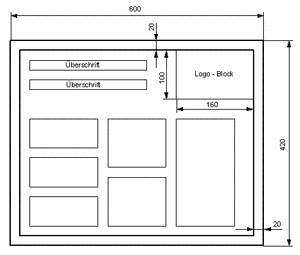
\includegraphics[keepaspectratio, width=9cm]{example_files/RTEmagicC_poster.jpg}
  \caption{Gestaltungsrichtlinie des Posters, Maße und Abstände}
  \label{fig:poster}
\end{figure}

\minisec{Gestaltung des Logo-Blocks}
Maße und Schriftgrößen siehe oben und in Abbildungen \ref{fig:poster} und \ref{fig:poster-logo-block}

\begin{figure}[ht]
  \centering
  
\includegraphics[keepaspectratio, width=9cm]{example_files/RTEmagicC_muster.jpg}
  \caption{Gestaltungsrichtlinie des Logo-Blocks des Posters}
  \label{fig:poster-logo-block}
\end{figure}


%%%%%%%%%%%%%%%%%%%%%%%%%%%%%%%%%%%%%%%%%%%%%%%%%%%%%%%%%%%%%%%%%%%%%%
\section{Informationsmittel zur Literaturrecherche}
\label{sec:InformationsmittelZurLiteraturrecherche}
%%%%%%%%%%%%%%%%%%%%%%%%%%%%%%%%%%%%%%%%%%%%%%%%%%%%%%%%%%%%%%%%%%%%%%

Wegen der ständig anwachsenden Zahl von Veröffentlichungen ist es angebracht, bei der Literaturrecherche rationelle Methoden anzuwenden.
Dafür stehen in den wissenschaftlichen Bibliotheken
\begin{compactitem}
  \item Sächsische Landesbibliothek -- Staats- und Universitätsbibliothek (SLUB)
  \item Fachbibliothek Elektrotechnik und Informationstechnik (FBE, DrePunct, Zellescher Weg 17)
\end{compactitem}
Informationsmittel zur Verfügung.

\begin{table*}[h]
  \centering
  \caption{Kataloge}
  \label{tab:Kataloge}
  \begin{tabular}{lll}%{p{4cm}p{4cm}p{4cm}}
    \toprule
    Bezeichnung     &                                                   & Standort  \\
    \midrule
    {\bfseries Kataloge}  & Alphabetischer Katalog                      & SLUB, FBE \\
                    & Sachkatalog                                       & SLUB, FBE \\
                    & Dissertationskatalog                              & SLUB, FBE \\
                    & Zeitschriftenkatalog                              & SLUB, FBE \\
                    & Zentralkatalog                                    & SLUB      \\
    \multicolumn{2}{l}{Bibliographien}                                  & SLUB, FBE \\
    \multicolumn{2}{l}{Firmenschriften/Prospekte/Wirtschaftsliteratur}  & SLUB      \\
    \multicolumn{2}{l}{Normen}                                          & SLUB, FBE \\
    \multicolumn{2}{l}{Dokumentations- und Referatedienste}             & SLUB, FBE \\
    \multicolumn{2}{l}{Patente}                                         & SLUB\\
    \bottomrule
  \end{tabular}
\end{table*}

\minisec{Rechnergestützte Recherche-Mittel}
\begin{compactitem}
  \item Rechnergestützter Katalog OPAC (Monographie-Bestand der SLUB)
  \item Recherchen in CD-ROM-Datenbanken verschiedener Hersteller (SLUB)
  \item IEEE-Dokumente: Aufsätze, Tagungsbandbeiträge etc. (Volltexte seit 1951 von Uni-IP)
  \item TOC Premier: Zeitschrifteninhaltsverzeichnisse führender Verlage weltweit (Literaturrecherche von Uni-IP)
  \item Datenbank FIZ Technik und Unterdatenbanken: (Literaturrecherche von Uni-IP)
  \item Online-Informationsdienst in kostenpflichtigen Datenbanken (SLUB)
  \item Internet
\end{compactitem}

%%%%%%%%%%%%%%%%%%%%%%%%%%%%%%%%%%%%%%%%%%%%%%%%%%%%%%%%%%%%%%%%%%%%%%
\section{Hilfestellung zum wissenschaftlichen Schreiben}
\label{sec:HilfestellungZumwissenschaftlichenSchreiben}
%%%%%%%%%%%%%%%%%%%%%%%%%%%%%%%%%%%%%%%%%%%%%%%%%%%%%%%%%%%%%%%%%%%%%%

\begin{itemize}
  \item \href{http://www.et.tu-dresden.de/ifa/fileadmin/user_upload/www_files/richtlinien_sa_da/Flyer_Wiss_Schreiben_Deutsch.pdf}{Wissenschaftlich Schreiben auf Deutsch ?!}
  \item \href{http://www.et.tu-dresden.de/ifa/fileadmin/user_upload/www_files/richtlinien_sa_da/Flyer_Wiss_Schreiben_Englisch.pdf}{Wissenschaftlich Schreiben auf Englisch ?!}
  \item \href{http://www.et.tu-dresden.de/ifa/fileadmin/user_upload/www_files/richtlinien_sa_da/Flyer_Wiss_Schreiben_Chinesisch.pdf}{Wissenschaftlich Schreiben auf Chinesisch ?!}
\end{itemize}

%%%%%%%%%%%%%%%%%%%%%%%%%%%%%%%%%%%%%%%%%%%%%%%%%%%%%%%%%%%%%%%%%%%%%%
\section[Installations- und Portierungsanleitung]{Spezielle Anforderungen an Installationsanleitung und Portierungsanleitung für Software}
\label{sec:SpezielleAnforderungenAnInstallationsanleitungUndPortierungsanleitungFuerSoftware}
%%%%%%%%%%%%%%%%%%%%%%%%%%%%%%%%%%%%%%%%%%%%%%%%%%%%%%%%%%%%%%%%%%%%%%

Das Ziel der Installation beschränkt sich auf das Ausführen der Software. Das Ziel der Portierung erweitert sich auf die Weiterentwicklung der Software. Dies beinhaltet i.A. auch eine Kompilierung der Software ohne jegliche Änderungen im Quellcode. Durch die Installationsanleitung und die Portierungsanleitung sollen unproblematische Installation und Portierung der Software auf die erforderliche Rechnerplattform sichergestellt werden.

\subsubsection*{Installationsanleitung}

Die Installationsanleitung ist eine klare, eindeutige und detaillierte Darstellung aller Handlungsschritte, die durchgeführt werden sollen, um die Software:

\begin{itemize}
  \item von einem (mitgelieferten) Datenträger (mit ausführbaren Datei(en), Konfigurationsdatei(en), Bibliothek(en) usw.),
  \item auf einer Rechnerplattform mit einer zur Ausführung erforderlichen Konfiguration (ggf. mit einer speziellen Programmierhardware, z.B. für FPGA)
\end{itemize}

zu installieren, sodass die Software ausgeführt werden kann. Die zur Ausführung erforderliche Konfiguration der Rechnerplattform ist hier zu beschreiben.

\subsubsection*{Portierungsanleitung}

Die Portierungsanleitung ist eine klare, eindeutige und detaillierte Darstellung aller Handlungsschritte, die durchgeführt werden sollen, um die Software:

\begin{itemize}
  \item von einem (mitgelieferten) Datenträger (mit Quelldatei(en), Konfigurationsdatei(en), Bibliothek(en) usw.),
  \item auf eine Rechnerplattform mit einer zur Entwicklung erforderlichen Konfiguration (ggf. mit einer speziellen Programmierhardware, z.B. für FPGA)
\end{itemize}

zu übertragen und auf dieser Rechnerplattform kompilieren, ausführen und weiterentwickeln zu können. Die zur Entwicklung erforderliche Konfiguration der Rechnerplattform ist hier zu beschreiben.

\subsubsection*{Beschreibung der erforderlichen Konfiguration der Rechnerplattform}

Die erforderliche Konfiguration der Rechnerplattform legt sowohl die Hardware als auch die Software (inkl. Betriebssystem(e) und ggf. Entwicklungssoftware) der Rechnerplattform fest, welche zur Ausführung bzw. zur Weiterentwicklung der Software erforderlich sind.

Die jeweilige erforderliche Konfiguration ist in der Installationsanleitung und in der Portierungsanleitung zu beschreiben. Falls dies in einem anderen Dokument erfolgt, soll ein eindeutiger Hinweis mit einem Verweis auf dieses Dokument eingefügt werden.

Die Softwarekomponenten der erforderlichen Konfiguration werden unter der Angabe von vollständigen Namen, Version(en) und bei Open Source Software von Bezugsquelle(n) spezifiziert. Die Installation dieser erforderlichen Software ist ebenfalls zu beschreiben. Verweise auf vorhandene Installationsanleitungen sind möglich, eventuelle ergänzende oder abweichende Schritte sind hier anzugeben.
